\section{Additional Figures}

\begin{figure}[h]
    \centering
    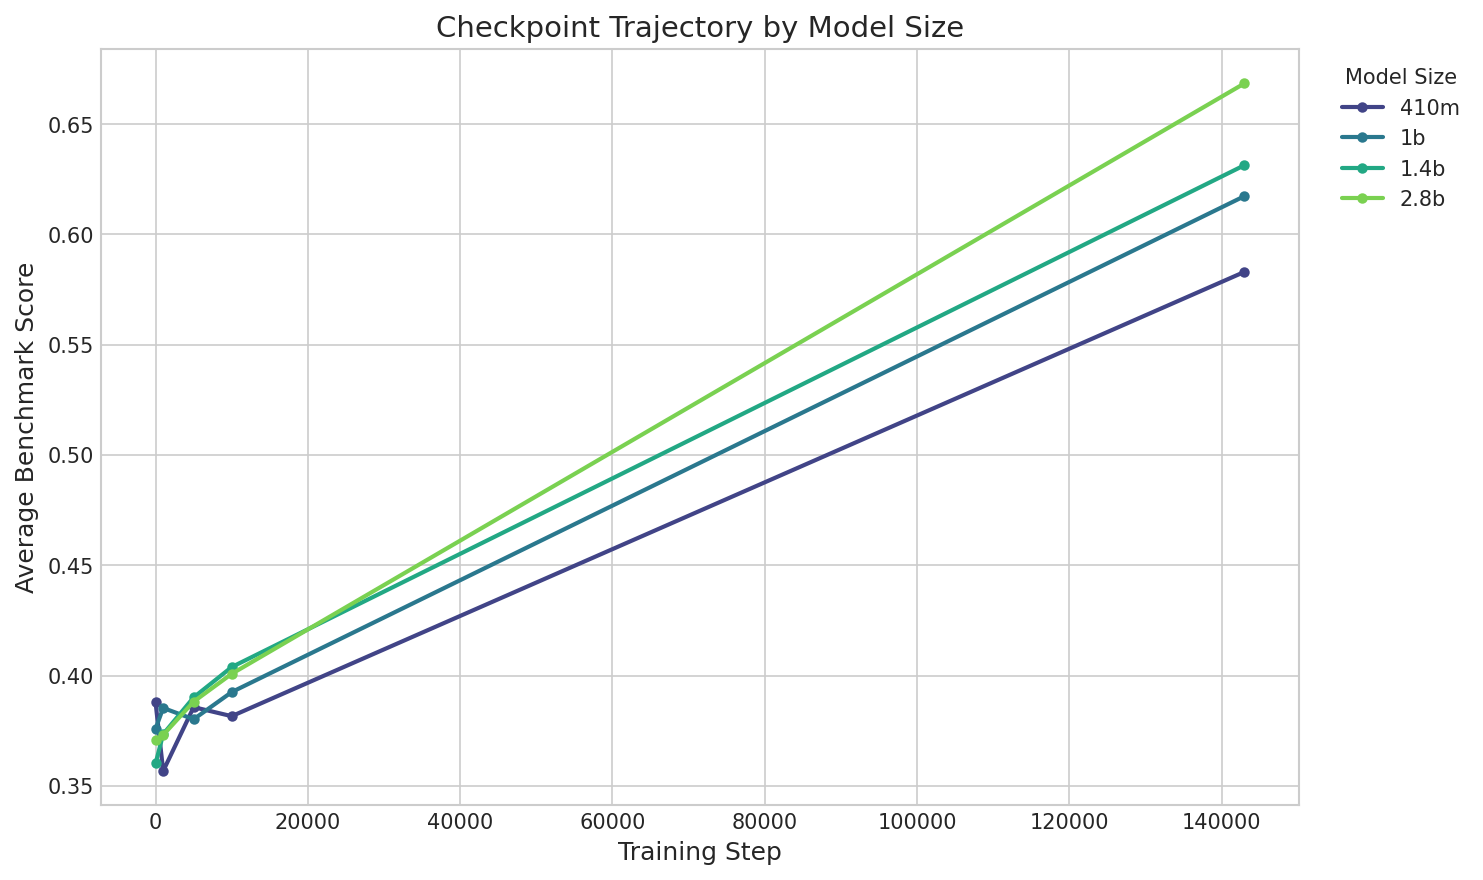
\includegraphics[width=\columnwidth]{figures/checkpoint_trajectory.png}
    \caption{Checkpoint trajectory visualization showing model performance evolution across training steps.}
    \label{fig:checkpoint_trajectory}
\end{figure}

\begin{figure}[h]
    \centering
    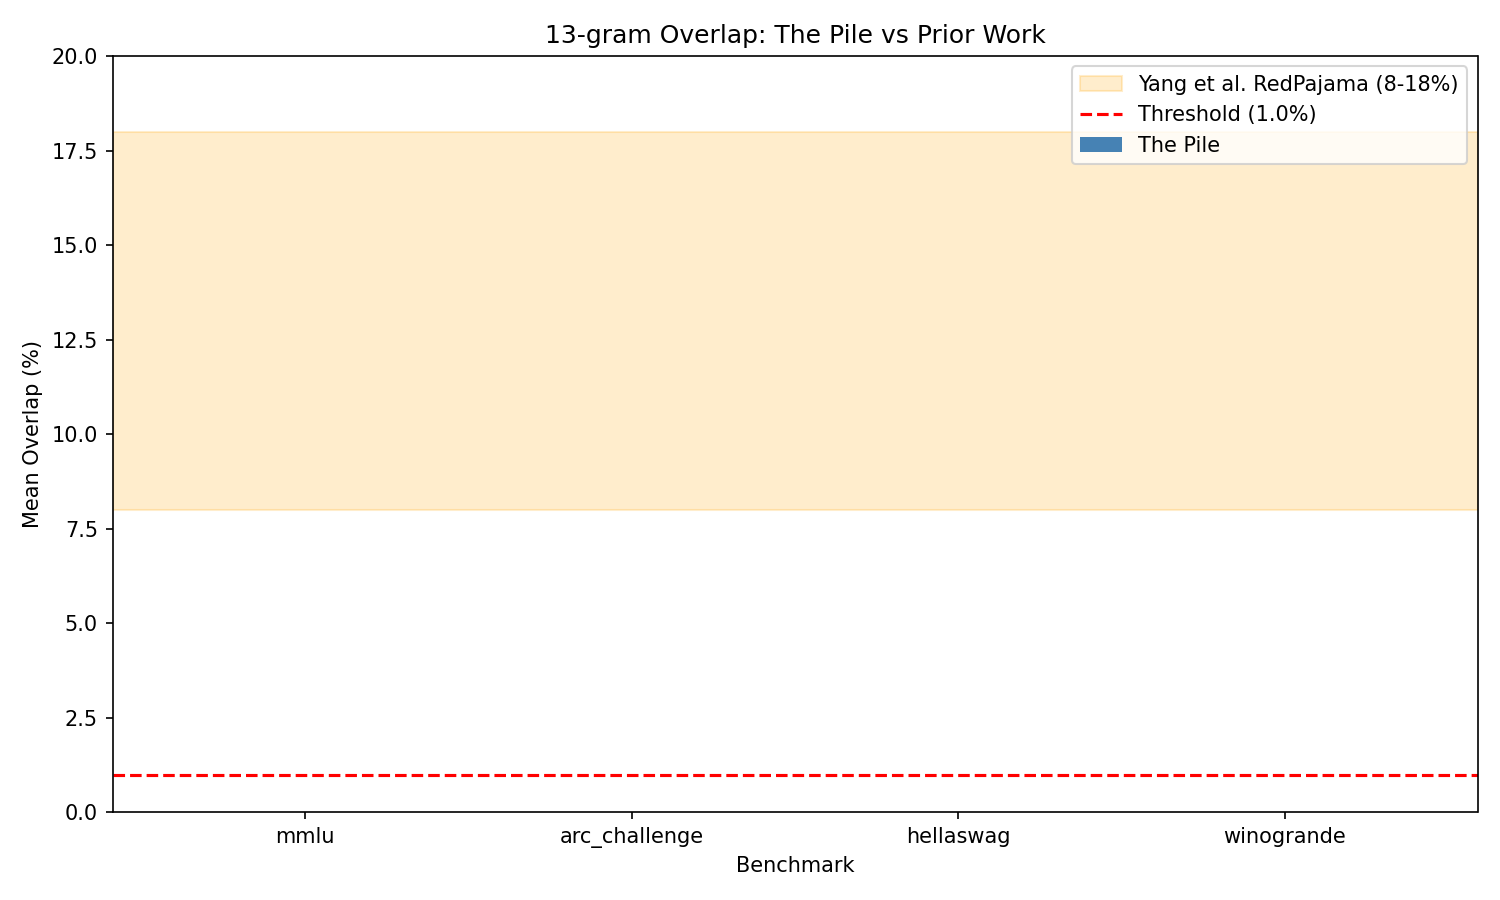
\includegraphics[width=\columnwidth]{figures/comparison_prior_work.png}
    \caption{Comparison with prior work on contamination detection methodologies.}
    \label{fig:comparison_prior_work}
\end{figure}

\begin{figure}[h]
    \centering
    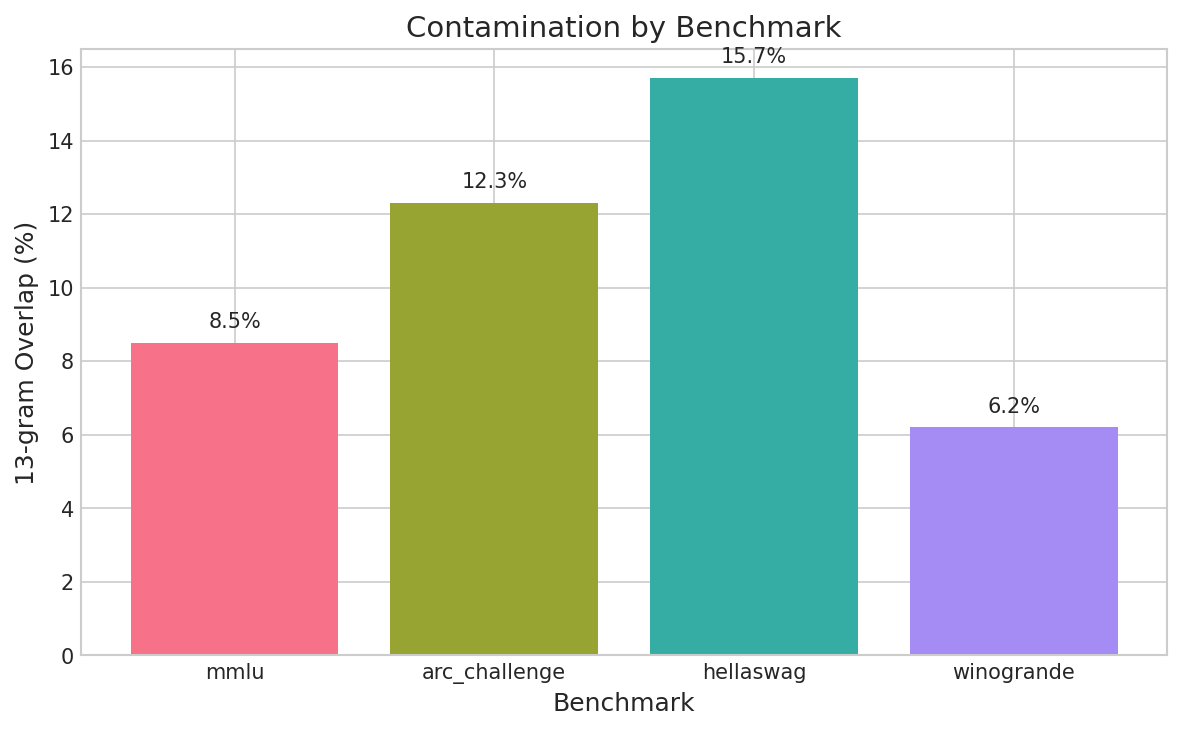
\includegraphics[width=\columnwidth]{figures/contamination_by_benchmark.png}
    \caption{Contamination levels across different benchmarks.}
    \label{fig:contamination_by_benchmark}
\end{figure}

\begin{figure}[h]
    \centering
    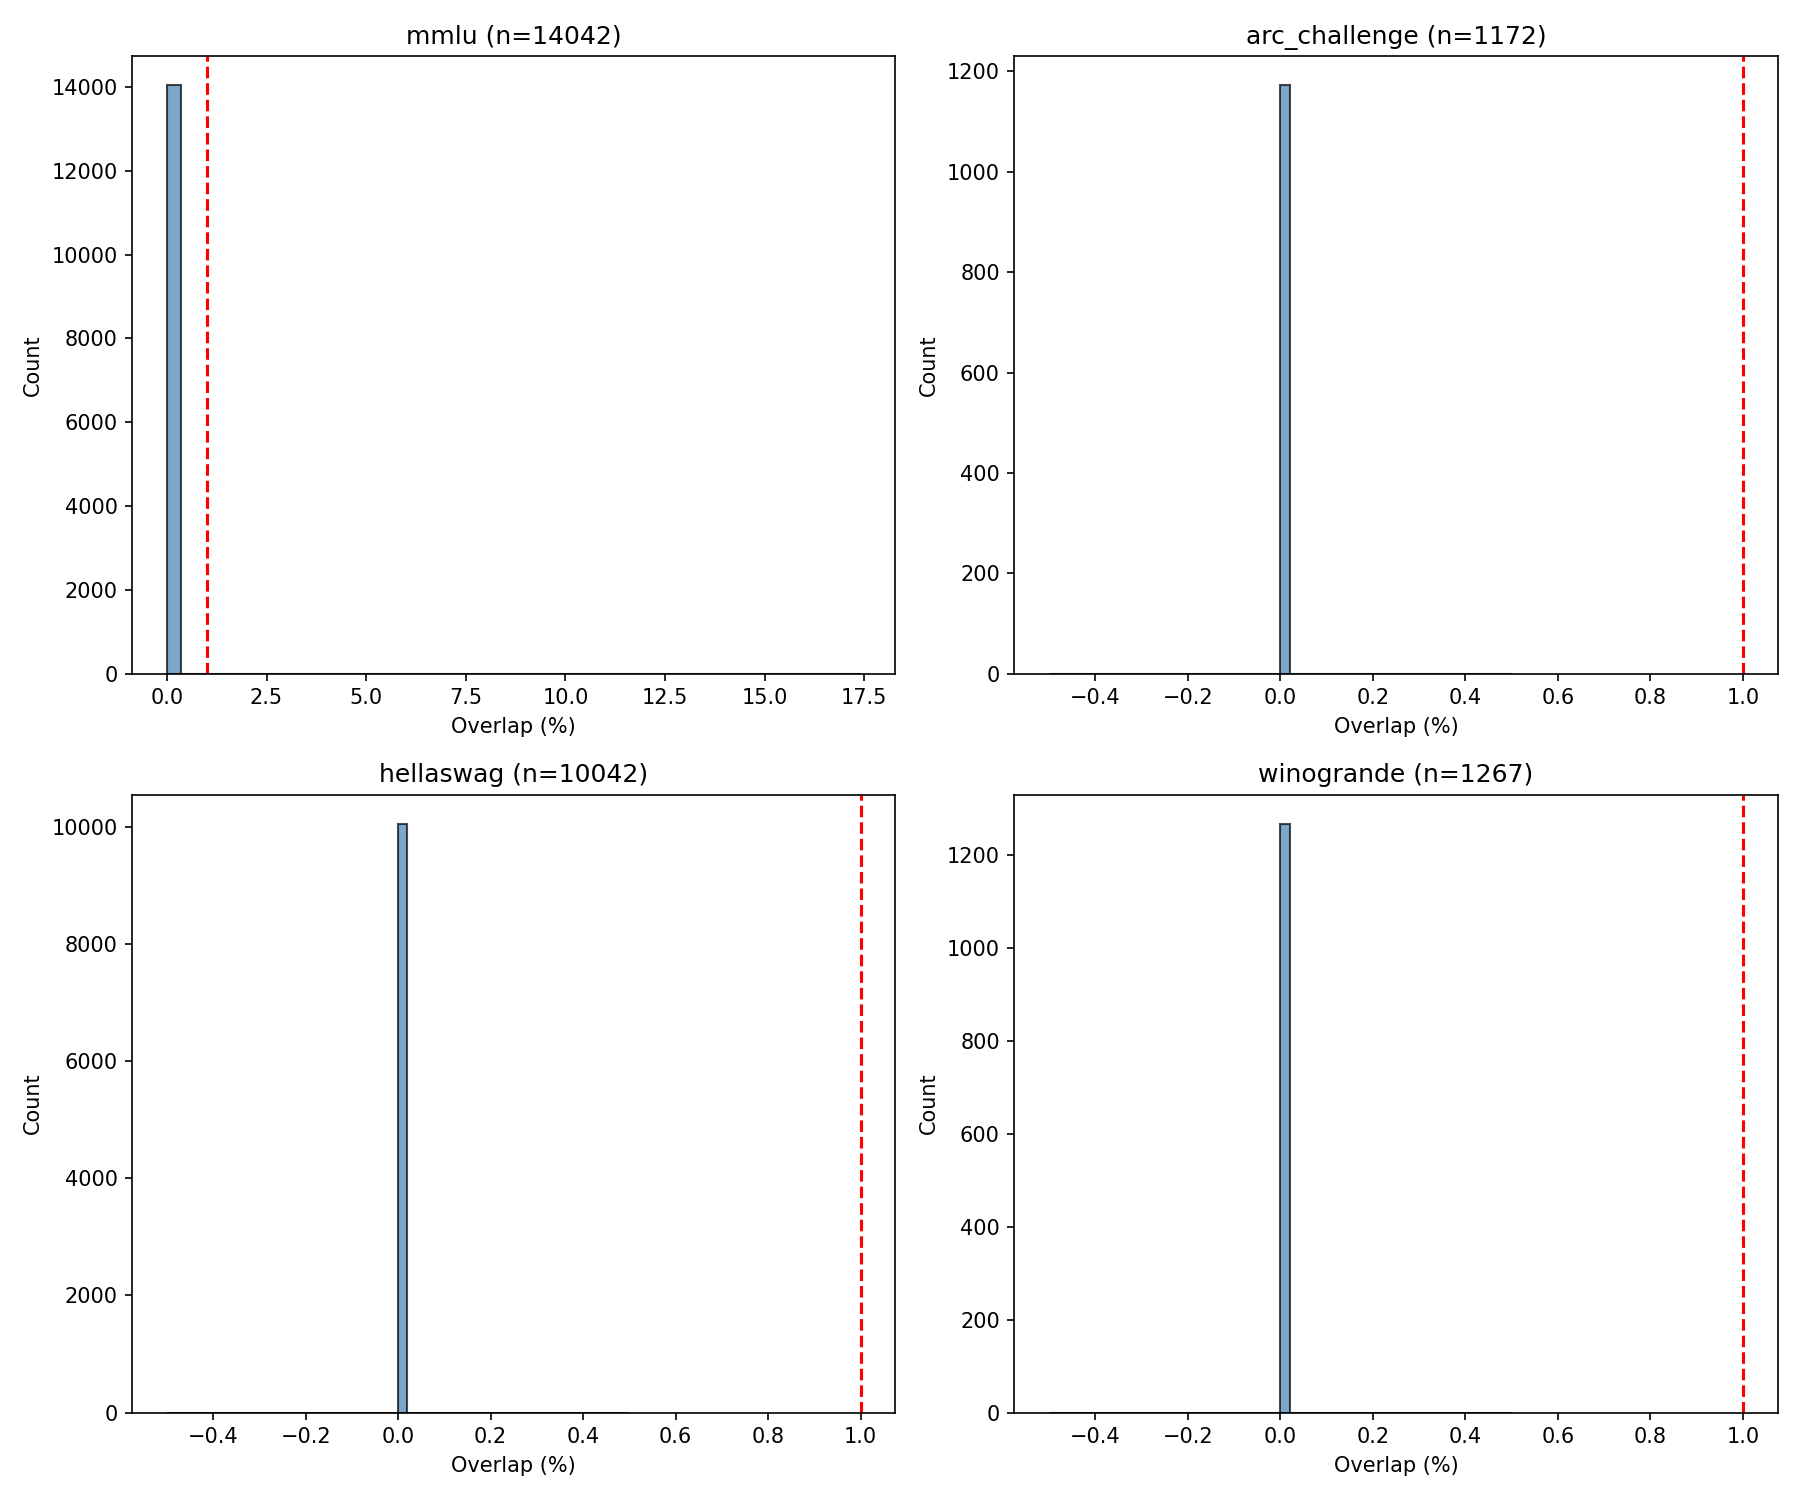
\includegraphics[width=\columnwidth]{figures/overlap_histograms.png}
    \caption{Distribution of n-gram overlap percentages across benchmark items.}
    \label{fig:overlap_histograms}
\end{figure}

\begin{figure}[h]
    \centering
    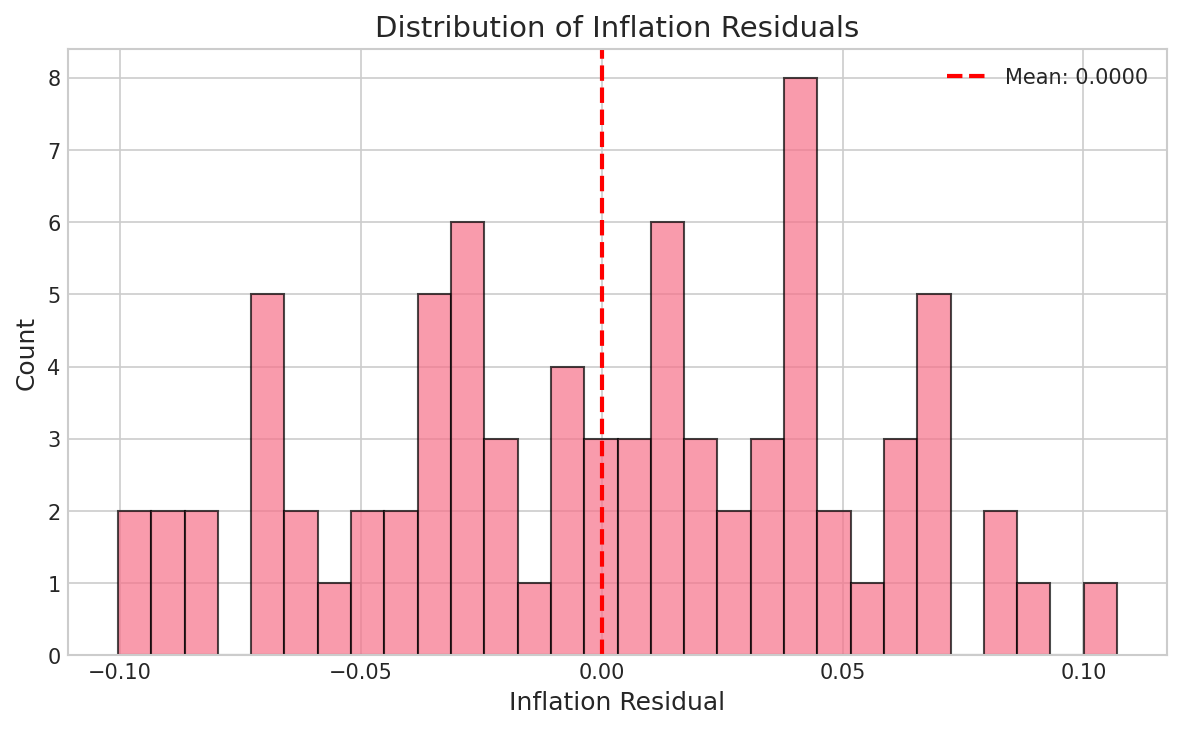
\includegraphics[width=\columnwidth]{figures/residual_distribution.png}
    \caption{Distribution of inflation residuals after capability detrending.}
    \label{fig:residual_distribution}
\end{figure}
